\documentclass{article}
\usepackage[utf8]{inputenc}
\usepackage[russian]{babel}
\usepackage{amsmath}
\usepackage[a4paper,margin=1in]{geometry}
\usepackage{titlesec}
\usepackage{graphicx}
\usepackage{listings}
\usepackage{caption}

\titleformat{\section}{\normalfont\Large\bfseries}{\Roman{section}}{1em}{}
\title{Отчёт по практическому заданию №1.}
\author{Козлов Кирилл 305 группа}
\date{\today}
\lstset{basicstyle=\ttfamily,breaklines=true,extendedchars=true}

\begin{document}

\maketitle

\newpage

\tableofcontents


\newpage

\section{Постановка задачи.}
\text{$\quad$}1. Вычислить таблицу значений функции \text{ $y = \cos(x/10)\cdot\arctan(x)$}  на сетке, полученной разбиением отрезка [0.5,1.5] на 20 равных частей:
\[ \text{$y_i = \cos(x_i/10)\cdot\arctan(x_i),\quad x_i = 0.5 + i{\cdot}h, \quad h = \frac{1.5-0.5}{20} ,\quad (i = 0,1,...,20) $}\]\\
\text{$\quad$}2. Построить 3 полинома \text{$ p_n(x) = a_{0}\cdot x^n + a_{1}\cdot x^{n-1} + ... + a_{n}$} последовательных степеней \text{$ n = 2, 3, 4$}, дающих наилучшее 
среднеквадратичное приближение \text{$f(x)$} на сетке \text{$x_i$} , т.е. для каждого n найти точку \text{$(a_{0},a_{1},...,a_{n})$} в \text{$R_{n+1}$}, в которой
достигается минимум функции \[ \Phi(a_{0},a_{1}, ... ,a_{n}) = \sum_{i=0}^{20}[y_i - p_{n}(x_{i})]^2\] 
Минимизацию \text{$\Phi(a_{0},a_{1}, ... ,a_{n})$} будем проводить усовершенствованным методом градиентного спуска 
- \textbf{\underline{метод сопряженных градиентов Флетчера-Ривса.}} 
В качестве начальной точки будем брать \text{$a_{0}^{(0)} = a_{1}^{(0)} = ... = a_{n}^{(0)} = 0. $} 
За меру точности приближения примем \[\triangle_{k+1} = \lVert x^{(k+1)}-x^{(k)}\rVert\] 
Процесс приближений заканчивается , если \text{$\triangle_{k} < \varepsilon$} ,где \text{$\varepsilon = 10^{-4}$} \\\\
\text{$\quad$}3. Для каждого из полученных таким образом \text{$p_n(x)$} вычислить \text{$y_{i}^{(n)} = p_n(x_{i})\quad (i = 0,1,...,20)$} 
и соответствующее среднеквадратическое отклонение:\[ \sigma_{n} = \sqrt{\frac{1}{21}\cdot\sum_{i=0}^{20}[y_i - p_{n}(x_{i})]^2} = \sqrt{\frac{\Phi_{min}}{21}}\]

\section{Метод спуска для отыскания минимума функции многих переменных(метод сопряженных градиентов Флетчера-Ривса).}
\text{$\quad$}1. Пусть требуется найти локальный минимум функции \[ \Phi(x) = \Phi(x_{1},x_{2}, ... ,x_{n})\] 
Выберем начальное приближение \text{$x^{(0)}$} и построим последовательность 
\text{$x^{(0)}, x^{(1)}, x^{(2)}, ... ,x^{(k)}, ...$}, в которой каждое очередное приближение 
\text{$x^{(k+1)}$} получается из предыдущего \text{$x^{(k)}$} "шагом" в направлении вектора \text{$v^{(k)}$}: \[ x^{(k+1)} = x^{(k)} + \lambda_{k}\cdot v^{(k)} \]
Величина шага управляется выбором \text{$\lambda_{k}$}. Обычно \text{$\lambda_{k}$} выбирается 
так, чтобы функция \[ \psi_{(k)} \equiv \Phi(x^{(k)} + \lambda\cdot v^{(k)}) \]
принимала наименьшее значение. 
Точность полученного приближения к минимуму обычно оценивается по величине отклонения двух соседних приближений \text{$x^{(k)}$} и 
\text{$x^{(k+1)}$} , например \[\triangle_{k+1} = \lVert x^{(k+1)}-x^{(k)}\rVert\] 
Процесс приближений заканчивается, если \text{$\triangle_{k}< \varepsilon$}, где \text{$\varepsilon$} - заданная точность. \\
\text{$\quad$}2. В методе Флетчера-Ривса направление спуска - вектор \text{$v^{(k)}$} - выбирается следующим образом:
\[ v^{(0)} = -grad\Phi(x^{(0)})\]
\[ v^{(k+1)} = -grad\Phi(x^{(k+1)}) + \beta_{k}\cdot v^{(k)}\] ,где
\[ \beta_{k} = \frac{|grad\Phi(x^{(k+1)})|^2}{|grad\Phi(x^{(k)})|^2} \quad (k = 0,1,2,...)\] 
Таким образом , на каждом шаге спуск несколько отклоняется от "скорейшего" в направлении предыдущего шага, что даёт 
некоторое ускорение сходимости вблизи точки минимума (когда близок к нулю \text{$grad \Phi(x)$}). 
В случае квадратичной функции \text{$\Phi(x)$} описываемые методы сходятся при любом выборе начального приближения.\text{$x^{(0)}$} \\ 
\text{$\quad$}3. Для нахождения \text{$\lambda_{k}$} на каждом шаге спуска нужно находить минимум функции одной переменной \text{$\psi_{k}(\lambda)$}, определяемой равенством \text{$\psi_{(k)} = \Phi(x^{(k)} + \lambda\cdot v^{(k)}) $}.
В общем случае для этого можно решать уравнение \text{$\frac{d\psi_{k}(\lambda)}{d\lambda} = 0$}, выражающее условие минимальности \text{$\psi_{k}(\lambda)$}. 
В нашем случае для минимальности функции \text{$\psi_{k}(\lambda)$} , \text{$\lambda $} выражается следующим образом:
\[\lambda = \frac{\sum_{i=0}^{20}(f(x_{i})\cdot V) - \sum_{i=0}^{20}(V( x_{1}^{(k)}\cdot x_{i}^{n} + x_{2}^{(k)}\cdot x_{i}^{n-1} + ... + x^{(k)}_{k} ))}{\sum_{i=0}^{20}(V^2)}\] , где 
\[ V = v_{1}^{(k)}\cdot x_{i}^{n} + v_{2}^{(k)}\cdot x_{i}^{n-1} + ... + v_{k}^{(k)}\] \\
\text{$\quad$}4. Для контроля за процессом сходимости спуска на каждом шаге удобно выдавать на печать величины:
k (номер шага),\text{$\quad$} \text{$\triangle_{k}$} , \text{$\quad$} \text{$g_{k} = |grad(\Phi(x^{k}))|$}. Метод спуска сходится к точке минимума \text{$\Phi(x^{k})$}, если: 
\[ 1. \quad\Phi(x^{k})\quad\text{убывает};\] 
\[ 2. \quad\text{$g_{k} \to 0$};\] 
\[ 3. \quad\triangle_{k} \to 0;\]
\newpage

\section{Блок-схема программы.}
\begin{figure}[h]
\centering
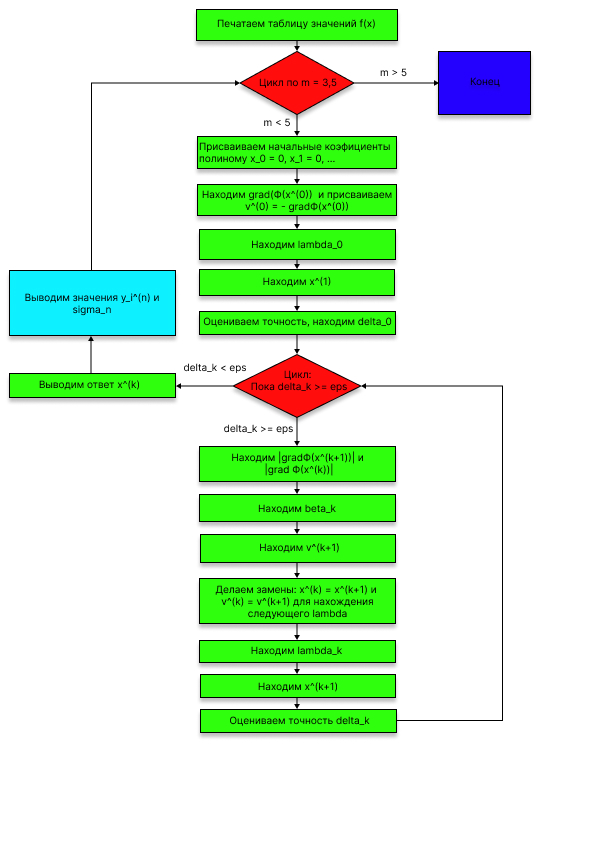
\includegraphics[height=1.1\textwidth]{algorythm.jpg}
\caption{Блок-схема программы}
\label{fig:myphoto}
\end{figure}
\newpage

\section{Программа решения задачи на Fortran.}
\lstinputlisting[language=Fortran]{task1.f90}
\newpage

\section{Тесты работы программы.}
\text{$\quad$} 1. Для функции \text{$y = \cos(x/10)\cdot\arctan(x)$}  на отрезке [0.5,1.5] получим следующие значения полиномов:
\[\text{2 степень полинома, коэфициенты: } a_{0} = -0.256448418 , a_{1} = 1.01533222 , a_{2} = 0.0225474089 \]
\[\text{3 степень полинома, коэфициенты: } a_{0} = 0.0746004581 , a_{1} = -0.480280489 , a_{2} = 1.22692657 , a_{3} = -0.0398121364 \]
\[\text{4 степень полинома, коэфициенты: } a_{0} = 0.115918584 , a_{1} = -0.392639726 , a_{2} = 0.198947981, a_{3} = 0.807098985 , a_{4} = 0.0528342798 \] 
Теперь проверим нашу программу на произвольном полиноме,допустим, 3 степени: \\
\text{$y = 1.122\cdot x^{3} - 0.213\cdot x^2 + 5.323\cdot x - 2.1231$}.Если подставить эту фукцию в нашу программу, то получатся коэфициенты:
\[\text{3 степень полинома, коэфициенты: } a_{0} = 1.12239671 , a_{1} = -0.213400945 , a_{2} = 5.32244205 , a_{3} = -2.12260127 \]
При этом значение \text{$|grad\Phi(x^{(k)})| \to 0$}. 

\section{Таблицы полученных результатов.}
\begin{table}[h]
    \centering
    \caption{Таблица значений полинома 2 степени}
    \begin{tabular}{|c|c|}
     \hline
     Величина & Значение \\
     \hline
     a0 & -0.256448418 \\
     a1 & 1.01533222 \\
     a2 & 0.0225474089 \\
     |grad(\text{$Ф(x^{5})$})| & 0.39869 \\
     \text{$\sigma_{2}$} & 0.00161 \\
     \hline
    \end{tabular}
\end{table}
\begin{table}[h]
    \centering
    \caption{Таблица значений полинома 3 степени}
    \begin{tabular}{|c|c|}
     \hline
     Величина & Значение \\
     \hline
     a0 & 0.0746004581 \\
     a1 & -0.480280489 \\
     a2 & 1.22692657 \\
     a3 & -0.0398121364 \\
     |grad(\text{$Ф(x^{(9)})$})| & 0.00810 \\
     \text{$\sigma_{3}$} & 0.00006 \\
     \hline
    \end{tabular}
\end{table}
\begin{table}[h]
    \centering
    \caption{Таблица значений полинома 4 степени}
    \begin{tabular}{|c|c|}
     \hline
     Величина & Значение \\
     \hline
     a0 & 0.115918584 \\
     a1 & -0.392639726 \\
     a2 & 0.198947981 \\
     a3 & 0.807098985 \\
     a4 & 0.0528342798 \\
     |grad(\text{$Ф(x^{(8)})$})| & 0.07443 \\
     \text{$\sigma_{4}$} & 0.00061 \\
     \hline
    \end{tabular}
\end{table}
\section{Перечень и характеристика всех ошибок, обнаруженных при прохождении задания.}
Единственной и самой обидной ошибкой было: при возведении полинома и функции в степень , вместо **(m-j) я написал **m-j и 
из-за этой ошибки в моей программе получались неверные ответы, градиент не стремился к нулю. Над этой проблемой я думал несколько дней. 
\end{document}
